\chapter{Formulación mediante elementos finitos}
\label{ch:elementos}

La descripción continua identifica puntos materiales, líneas de referencia y
orientaciones de sección sin introducir nodos. La discretización constituye un
paso posterior: sustituye los campos desconocidos por aproximaciones definidas
mediante un número finito de parámetros. Por ello, un nodo no es una partícula
adicional del cuerpo ni una unión física necesariamente existente. Es una
estación de interpolación de la línea de referencia. Una unión entre cuerpos,
en cambio, requiere una condición cinemática o una ley mecánica específica.

Este capítulo desarrolla la especialización a elementos rectos de viga de
Timoshenko con dos nodos. Se separan la interpolación de los campos, las
propiedades que relacionan deformaciones y resultantes, y las restricciones
entre componentes. Los fundamentos de aproximación y ensamblaje corresponden
al método de elementos finitos \cite{reddy}; la descripción de vínculos rígidos
se inscribe en la cinemática de sistemas multicuerpo \cite{shabana}. Las fórmulas
cerradas corresponden a elementos rectos de propiedades constantes, con
extensión, torsión y flexión con deformación por cortante.

\section{Del cuerpo continuo a la malla de vigas}

Sea $S$ la coordenada material longitudinal de la torre o de una pala en la
configuración de referencia. Se divide su intervalo en subintervalos
$[S_I,S_J]$, de longitud $L=S_J-S_I>0$ para el elemento recto considerado.
Dentro de cada elemento se emplea $s=S-S_I\in[0,L]$. La discretización puede
aproximar mediante segmentos una línea inicialmente curva, pero las expresiones
cerradas siguientes corresponden a cada segmento recto, no a un elemento curvo
exacto. Los cambios de geometría o propiedades deben ser representados mediante
la partición o mediante una formulación que los admita explícitamente.

La figura~\ref{fig:continuo-malla} distingue la línea material continua de su partición en elementos; los nodos parametrizan la aproximación del movimiento.

\begin{figure}[htbp]
\centering
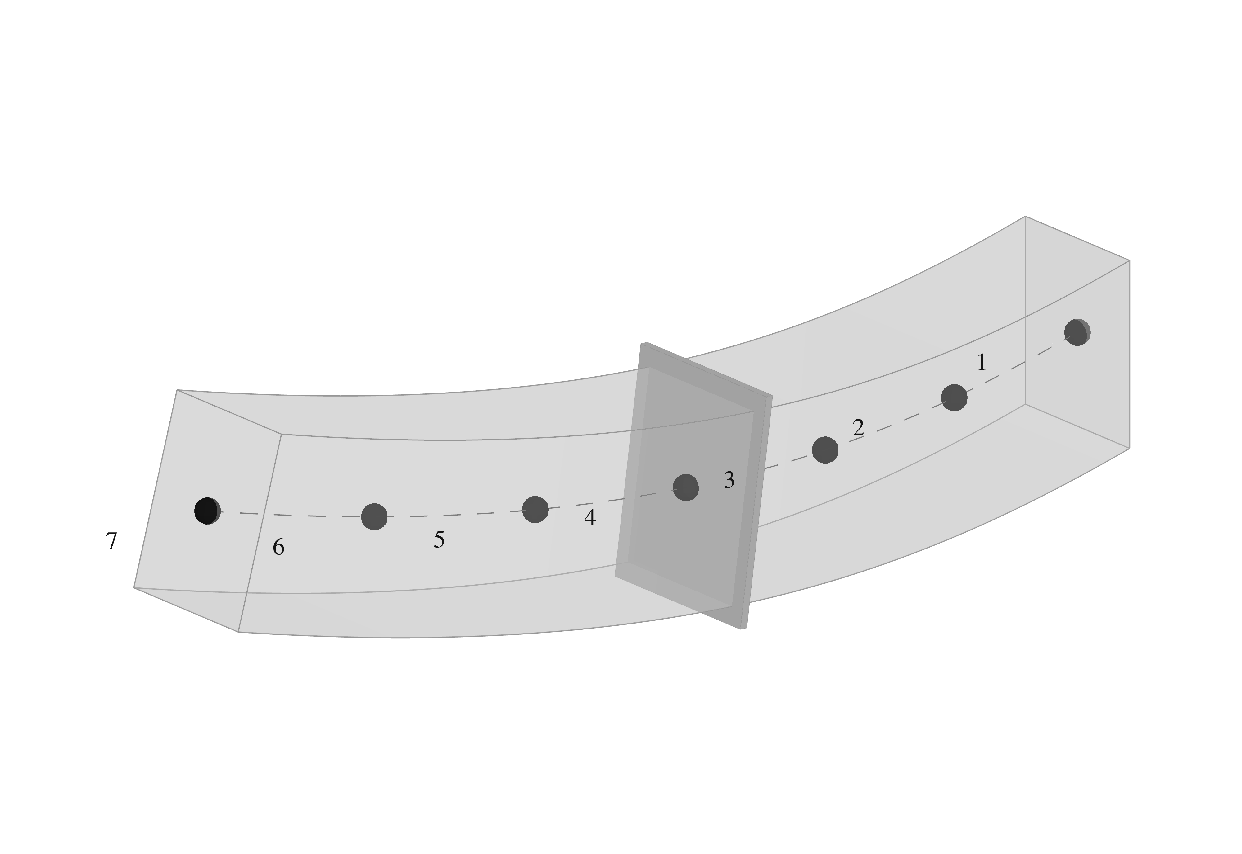
\includegraphics[width=.96\linewidth,height=.40\textheight,keepaspectratio]{figures/tecplot/concept_continuo-malla.pdf}
\caption[Descripción continua y discretización]{Envolvente de una viga, línea material de referencia y nodos de una partición espacial. Los números siguen el orden material de los nodos. El movimiento de la sección señalada se recupera mediante las coordenadas nodales. La superficie es ilustrativa y no representa elementos sólidos.}\label{fig:continuo-malla}
\end{figure}

En componentes locales se agrupan las perturbaciones de un nodo como
\begin{equation}
 \vct q_i^e=[u_{1i},u_{2i},u_{3i},\theta_{1i},\theta_{2i},\theta_{3i}]^{\tr},
 \qquad
 \vct q_e=[(\vct q_I^e)^{\tr},(\vct q_J^e)^{\tr}]^{\tr}.
\end{equation}
El superíndice $e$ indica componentes en la base local del elemento. Existen
doce coordenadas elementales antes de ensamblar e imponer vínculos: tres
traslaciones y tres pequeñas rotaciones por nodo. No son doce movimientos
independientes después de imponer un empotramiento o de identificar una raíz
con un cubo rígido. Tampoco incluyen el azimut nominal prescrito del rotor
como una incógnita adicional.

La hipótesis de Timoshenko permite que la normal a la sección y la tangente a
la línea deformada difieran. Se retienen extensión, dos deformaciones por
cortante, torsión y dos curvaturas. No se incorporan como incógnitas
independientes el alabeo de la sección, su distorsión en el plano o modos
locales de una pared. La reducción a viga debe interpretarse con estas
delimitaciones, aunque las propiedades seccionales procedan de un cálculo
tridimensional más detallado.

La figura~\ref{fig:coordenadas-nodo} separa las coordenadas de traslación de las coordenadas angulares de un nodo. Cada una multiplica una dirección local definida; la orientación del elemento permite después expresar todas en la base de ensamblaje. Una coordenada angular nodal describe el giro de la sección, no una pendiente impuesta de la línea.

\begin{figure}[htbp]
\centering
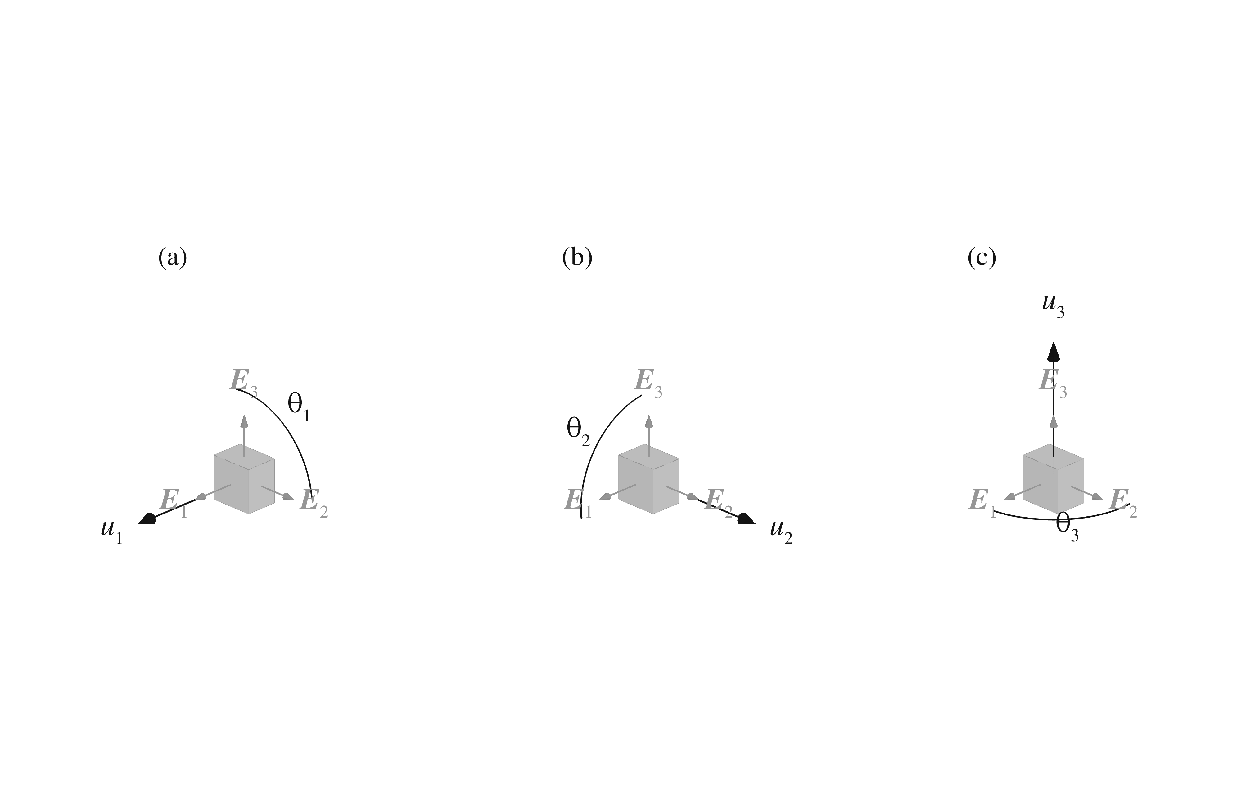
\includegraphics[width=.96\linewidth,height=.40\textheight,keepaspectratio]{figures/tecplot/concept_coordenadas-nodo.pdf}
\caption[Coordenadas de traslación y rotación de un nodo]{Las seis coordenadas de un nodo se organizan por dirección: (a) $u_1,\theta_1$, (b) $u_2,\theta_2$ y (c) $u_3,\theta_3$. La flecha recta representa una traslación y el arco una rotación alrededor del eje correspondiente. Las amplitudes se amplían y no constituyen una respuesta simultánea calculada.}\label{fig:coordenadas-nodo}
\end{figure}

\section{Interpolación y medidas de deformación}

El campo seccional aproximado se escribe
\begin{equation}
 \vct\eta(s)=
 [u_1,u_2,u_3,\theta_1,\theta_2,\theta_3]^{\tr}
 =\ten N(s)\vct q_e.
 \label{eq:fe-campo}
\end{equation}
Las traslaciones tienen dimensión de longitud y las rotaciones son
adimensionales. En consecuencia, algunas entradas de $\ten N$ que convierten
una rotación nodal en desplazamiento llevan dimensiones de longitud. No debe
interpretarse toda la matriz como una colección de funciones adimensionales.

En la aproximación lineal alrededor de una referencia recta, con ejes
dextrógiros y eje 1 longitudinal,
\begin{equation}
 \vct\varepsilon=
 \begin{bmatrix}u_{1,s}\\u_{2,s}-\theta_3\\u_{3,s}+\theta_2\\
 \theta_{1,s}\\\theta_{2,s}\\\theta_{3,s}\end{bmatrix}
 =\mathcal D\vct\eta=\ten B(s)\vct q_e,
 \qquad \ten B=\mathcal D\ten N.
 \label{eq:fe-strain}
\end{equation}
Aquí $\mathcal D$ es un operador diferencial explícito: deriva los campos
respecto de $s$ y combina las rotaciones con las pendientes transversales.
Las tres primeras entradas son deformaciones adimensionales y las tres
últimas tienen dimensión de inverso de longitud. La coexistencia de ambos
tipos explica las diferentes unidades de los bloques de rigidez seccional.

La interpolación más simple utiliza
$N_I=1-s/L$, $N_J=s/L$ y
$\ten N_{\rm lin}=[N_I\Id_6,N_J\Id_6]$. Por ejemplo,
\begin{equation}
 \gamma_2=\frac{u_{2J}-u_{2I}}{L}-N_I\theta_{3I}-N_J\theta_{3J}.
\end{equation}
La derivada del desplazamiento es constante, mientras que la rotación es
lineal. Cuando la viga se hace esbelta, imponer cortante prácticamente nulo en
todo el elemento restringe excesivamente esa combinación y puede producir
\emph{bloqueo por cortante}: la aproximación resulta artificialmente rígida.
No se trata de una propiedad física del material. Una opción es integrar
selectivamente la energía de cortante; otra es utilizar interpolaciones
compatibles con la solución del elemento. Ambas opciones son formulaciones
distintas y no deben combinarse sin justificar la operación.

La figura~\ref{fig:interpolacion-lineal} ilustra el significado de las funciones $N_I$ y $N_J$. En cada extremo se recupera exactamente el valor nodal correspondiente. En el interior, el valor se calcula mediante una combinación ponderada; no se introduce una nueva incógnita en cada sección. Esta ilustración corresponde a la interpolación lineal recién definida, no a las funciones cerradas de flexión que se deducen a continuación.

\begin{figure}[htbp]
\centering
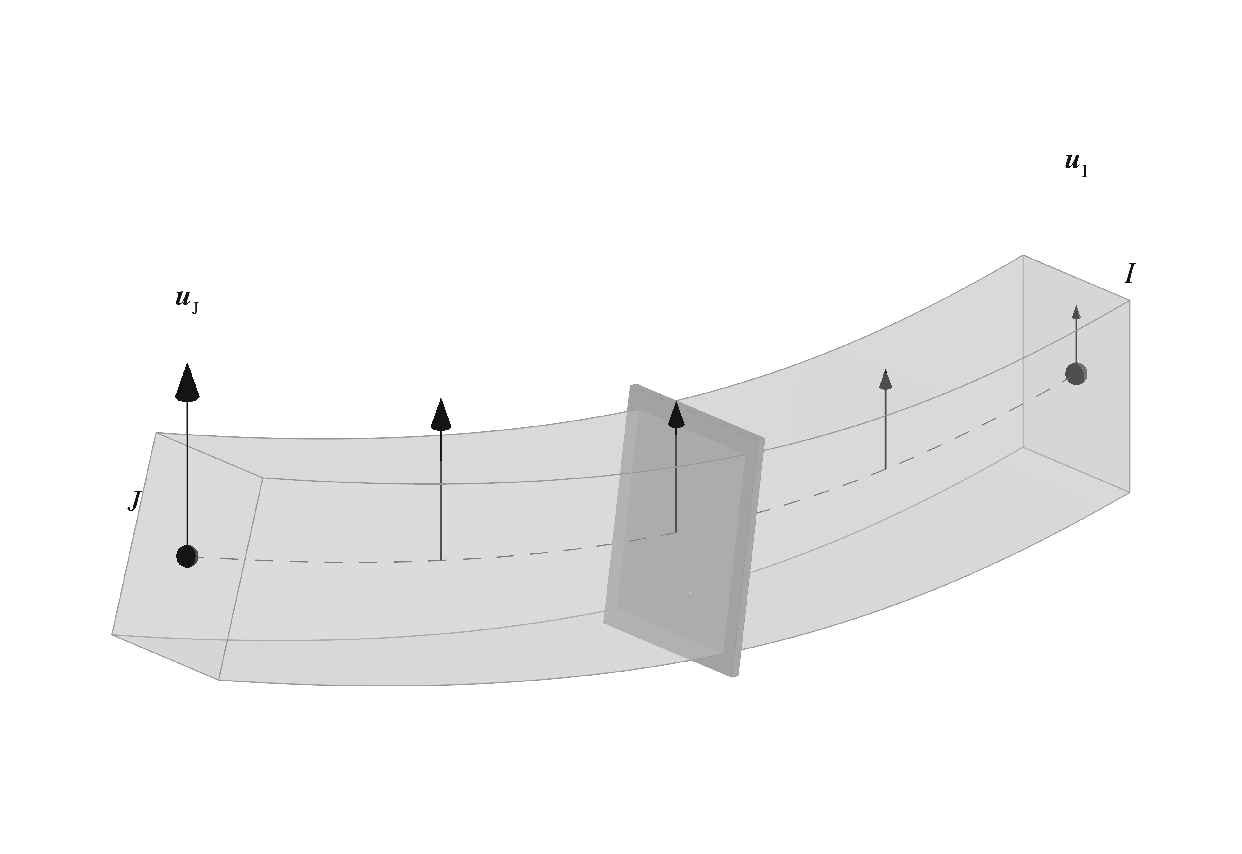
\includegraphics[width=.96\linewidth,height=.40\textheight,keepaspectratio]{figures/tecplot/concept_interpolacion-lineal.pdf}
\caption[Interpolación entre valores nodales]{Interpolación de un campo de desplazamientos entre los valores nodales $\vct u_I$ y $\vct u_J$. Las flechas intermedias ilustran $\vct u(S)=N_I(S)\vct u_I+N_J(S)\vct u_J$. La línea curva y la envolvente son esquemáticas; las expresiones elementales cerradas del texto corresponden a segmentos rectos.}\label{fig:interpolacion-lineal}
\end{figure}

\section{Especialización de propiedades constantes: interpolación cerrada}

La interpolación se obtiene de la solución estática homogénea de la viga de
Timoshenko, con propiedades constantes y desacopladas en cada elemento.
En el plano $(1,2)$ intervienen $EI_3$ y
$GA_{s2}$; se definen
\begin{equation}
 \phi_2=\frac{12EI_3}{GA_{s2}L^2},\quad
 \zeta=\frac{s}{L},\quad
 \vct p=[1,\zeta,\zeta^2,\zeta^3],\quad
 \vct d_2=[u_{2I},\theta_{3I},u_{2J},\theta_{3J}]^{\tr}.
\end{equation}
Para obtener las funciones de interpolación se considera primero un tramo sin carga distribuida. En el plano $(1,2)$, sus ecuaciones de equilibrio y constitutivas son
\begin{equation}
 n_2'=0,\qquad m_3'+n_2=0,\qquad
 n_2=GA_{s2}(u_2'-\theta_3),\qquad m_3=EI_3\theta_3'.
\end{equation}
Con propiedades constantes, la fuerza cortante $n_2$ es constante, el momento $m_3$ es lineal, la rotación $\theta_3$ es cuadrática y el desplazamiento $u_2$ es cúbico. Las cuatro constantes independientes se determinan imponiendo los valores de $u_2$ y $\theta_3$ en ambos extremos. La expresión matricial que sigue reúne esa solución en términos de las cuatro coordenadas nodales.

El parámetro $\phi_2$ cuantifica la contribución del cortante en relación con
la flexión para la longitud del elemento. Las áreas $A_{s2}$ y $A_{s3}$ son
áreas efectivas: si incluyen factores de corrección, estos no vuelven a
multiplicarse. Para un valor genérico $\phi$, sean
\begin{equation}
 \ten C_v=\frac{1}{1+\phi}
 \begin{bmatrix}
 1+\phi&0&0&0\\
 -\phi&L(1+\phi/2)&\phi&-L\phi/2\\
 -3&-L(2+\phi/2)&3&-L(1-\phi/2)\\
 2&L&-2&L
 \end{bmatrix},
\end{equation}
\begin{equation}
 \ten C_r=\frac{1}{1+\phi}
 \begin{bmatrix}
 0&1+\phi&0&0\\
 -6/L&-(4+\phi)&6/L&-(2-\phi)\\
 6/L&3&-6/L&3\\
 0&0&0&0
 \end{bmatrix}.
\end{equation}
Entonces $u_2=\vct p\ten C_v\vct d_2$ y
$\theta_3=\vct p\ten C_r\vct d_2$, usando $\phi=\phi_2$.
Estas funciones reproducen las coordenadas en ambos extremos y permiten
pendiente y rotación diferentes. La palabra ``exacta'' se refiere a la
solución estática homogénea del elemento recto de propiedades constantes que
genera estas funciones; no afirma que una malla finita reproduzca exactamente
todos los campos dinámicos o todas las cargas distribuidas.

En el plano $(1,3)$ se utiliza
\begin{equation}
 \phi_3=\frac{12EI_2}{GA_{s3}L^2},\quad
 \vct d_3=[u_{3I},\theta_{2I},u_{3J},\theta_{2J}]^{\tr},\quad
 \ten S_- =\diag(1,-1,1,-1),
\end{equation}
\begin{equation}
 u_3=\vct p\ten C_v\ten S_-\vct d_3,\qquad
 \theta_2=-\vct p\ten C_r\ten S_-\vct d_3,
 \qquad \phi=\phi_3.
\end{equation}
Los signos provienen de $\gamma_3=u_{3,s}+\theta_2$ y de la orientación de la
base, no de una diferencia física entre ambos planos. Finalmente, $u_1$ y
$\theta_1$ se interpolan con $N_I,N_J$. Estas seis relaciones definen todas
las entradas de $\ten N$; aplicar \eqref{eq:fe-strain} determina $\ten B$.

\section{Rigidez, masa y cargas elementales}

\subsection{Balance elemental y trabajo virtual}

Antes de construir matrices, se establece qué ecuaciones se aproximan. Sean
$\vct n(s)$ la fuerza interna de sección, $\vct m(s)$ el momento interno,
$\vct p(s)$ la fuerza externa por longitud y $\vct\ell(s)$ el momento externo
por longitud. Todos se expresan en la misma base local. Se adopta
\begin{equation}
 \vct t_s=\begin{bmatrix}\vct n\\\vct m\end{bmatrix}
 =\mathsf C_s\vct\varepsilon,
 \qquad
 \vct f_s=\begin{bmatrix}\vct p\\\vct\ell\end{bmatrix},
\end{equation}
donde $\mathsf C_s$ es la matriz seccional definida en el capítulo anterior.
El vector $\vct\ell$ no es una resultante interna: representa, por ejemplo,
un momento aerodinámico distribuido. Esta distinción evita confundir unidades
y acciones que intervienen en lados diferentes del balance.

Una variación virtual $\delta\vct\eta=[\delta\vct u^{\tr},
\delta\vct\theta^{\tr}]^{\tr}$ es un campo arbitrario compatible con los
vínculos homogéneos; no es una derivada temporal ni el movimiento real durante
un intervalo de tiempo. En esta subsección el símbolo $\delta$ denota la
variación de prueba. Las variaciones de deformación son
\begin{equation}
 \delta\vct\gamma=\delta\vct u_{,s}
 +\vct e_1\times\delta\vct\theta,
 \qquad
 \delta\vct\kappa=\delta\vct\theta_{,s}.
\end{equation}
Por tanto, el trabajo virtual interno toma la forma
\begin{align}
 \delta W_{\rm int}
 &=\int_0^L(\delta\vct\gamma\cdot\vct n
       +\delta\vct\kappa\cdot\vct m)\,\dd s\nonumber\\
 &=[\delta\vct u\cdot\vct n+
       \delta\vct\theta\cdot\vct m]_0^L\nonumber\\
 &\quad-\int_0^L\left[\delta\vct u\cdot\vct n_{,s}
       +\delta\vct\theta\cdot
       (\vct m_{,s}+\vct e_1\times\vct n)\right]\dd s.
 \label{eq:fe-partes}
\end{align}
La integración por partes revela el término de equilibrio de momentos
$\vct e_1\times\vct n$. Este término es precisamente la contraparte estática
del cortante de Timoshenko. No aparece al tratar traslaciones y rotaciones
como campos completamente independientes de la medida de deformación.

Sean $\vct i_u$ y $\vct i_\theta$ las resultantes inerciales por longitud.
El principio de trabajo virtual dinámico establece
\begin{equation}
 \int_0^L\delta\vct\varepsilon^{\tr}\vct t_s\,\dd s
 +\int_0^L\delta\vct\eta^{\tr}
        \begin{bmatrix}\vct i_u\\\vct i_\theta\end{bmatrix}\dd s
 =\int_0^L\delta\vct\eta^{\tr}\vct f_s\,\dd s
 +\delta W_{\partial e}.
 \label{eq:fe-debil}
\end{equation}
Para variaciones nulas en los extremos, \eqref{eq:fe-partes} conduce a los
balances locales
\begin{equation}
 \vct n_{,s}+\vct p=\vct i_u,\qquad
 \vct m_{,s}+\vct e_1\times\vct n+\vct\ell=\vct i_\theta.
\end{equation}
En los extremos libres de condiciones esenciales, el término de borde
identifica fuerzas y momentos aplicados: $(-\vct n,-\vct m)$ en $s=0$ y
$(\vct n,\vct m)$ en $s=L$. En un desplazamiento o giro impuesto, la variación
correspondiente se anula y la reacción se recupera posteriormente del
residual. Así se distinguen condiciones esenciales y naturales sin imponer
ambas a una misma coordenada de extremo.

Para pequeñas perturbaciones alrededor de una referencia estacionaria, sin
giro nominal y con base fija, las inercias son
$[\vct i_u^{\tr},\vct i_\theta^{\tr}]^{\tr}
=\mathsf M_s\ddot{\vct\eta}$, donde $\mathsf M_s$ es la matriz espacial del
capítulo anterior. El caso rotatorio incorpora términos adicionales de
transporte y velocidad; no se obtiene omitiéndolos en esta expresión
estacionaria. Sustituyendo $\vct\eta=\ten N\vct q_e$ y
$\delta\vct\eta=\ten N\delta\vct q_e$ en \eqref{eq:fe-debil}, para
$\ten N$ independiente del tiempo, se obtiene
\begin{equation}
 \delta\vct q_e^{\tr}
 (\ten M_e\ddot{\vct q}_e+\ten K_e\vct q_e
       -\vct f_e-\vct f_{\partial e})=0.
\end{equation}
La arbitrariedad de las coordenadas virtuales admisibles produce las
ecuaciones nodales. La forma débil es, por consiguiente, el vínculo entre los
balances continuos y las matrices que siguen; la energía elástica es una
representación equivalente de la contribución interna cuando
$\mathsf C_s$ es simétrica.

\subsection{Matrices elementales y cargas consistentes}

Si $\mathsf C_s$ es la matriz constitutiva seccional en la base local, la energía
elástica y su matriz elemental son
\begin{equation}
 U_e=\frac12\int_0^L\vct\varepsilon^{\tr}\mathsf C_s\vct\varepsilon\,\dd s
 =\frac12\vct q_e^{\tr}\ten K_e\vct q_e,
 \qquad
 \ten K_e=\int_0^L\ten B^{\tr}\mathsf C_s\ten B\,\dd s.
\end{equation}
Para $\mathsf C_s=\diag(EA,GA_{s2},GA_{s3},GJ_t,EI_2,EI_3)$, la extensión y la
torsión aportan, respectivamente,
\begin{equation}
 \ten K_{\rm ax}=\frac{EA}{L}\begin{bmatrix}1&-1\\-1&1\end{bmatrix},
 \qquad
 \ten K_{\rm tor}=\frac{GJ_t}{L}\begin{bmatrix}1&-1\\-1&1\end{bmatrix}.
\end{equation}
Se insertan en los índices $(1,7)$ y $(4,10)$ de $\vct q_e$. Para cada plano,
con sus valores de $EI$, $GA_s$ y $\phi=12EI/(GA_sL^2)$, se definen
\begin{equation}
 a=\frac{12EI}{L^3(1+\phi)},\quad b=\frac{6EI}{L^2(1+\phi)},\quad
 c=\frac{(4+\phi)EI}{L(1+\phi)},\quad d=\frac{(2-\phi)EI}{L(1+\phi)}.
\end{equation}
La contribución de flexión y cortante es
\begin{equation}
 \ten K_{\rm fl}=\begin{bmatrix}
 a&\sigma b&-a&\sigma b\\
 \sigma b&c&-\sigma b&d\\
 -a&-\sigma b&a&-\sigma b\\
 \sigma b&d&-\sigma b&c
 \end{bmatrix}.
\end{equation}
Se emplea $\sigma=1$, $EI=EI_3$ en los índices $(2,6,8,12)$ y
$\sigma=-1$, $EI=EI_2$ en $(3,5,9,11)$. Los cuatro bloques construyen la
matriz completa. Para una sección acoplada se conserva la integral general y
se elige una interpolación adecuada; no basta con agregar arbitrariamente
entradas a estos bloques desacoplados.

La masa seccional $\mathsf M_s$, construida con masa por longitud, tensor
centroidal y excentricidad, produce la matriz consistente
\begin{equation}
 \ten M_e=\int_0^L\ten N^{\tr}\mathsf M_s\ten N\,\dd s.
 \label{eq:fe-masa}
\end{equation}
``Consistente'' significa que se utiliza el mismo campo cinemático que
describe el movimiento. No implica concentrar toda la masa en los nodos. La
inercia rotacional permanece aunque el cortante tienda a cero; ese límite
dinámico corresponde a una viga con inercia rotacional, y no automáticamente
al modelo clásico de Euler--Bernoulli sin ella. Con propiedades constantes,
los productos polinómicos de la masa tienen grado máximo seis y cuatro puntos
de Gauss los integran exactamente. Si las propiedades varían, esta afirmación
de exactitud ya no se deduce únicamente del grado de $\ten N$.

Una distribución de fuerza $\vct p$ y momento $\vct\ell$ por longitud genera
\begin{equation}
 \vct f_e=\int_0^L\ten N^{\tr}
 \begin{bmatrix}\vct p\\\vct\ell\end{bmatrix}\dd s.
\end{equation}
Esta equivalencia se establece por igualdad de trabajo virtual, no por un
reparto intuitivo entre extremos. Si la carga depende de la configuración o
velocidad, también deben evaluarse sus derivadas al linealizar las ecuaciones.

\section{Cambio de componentes y ensamblaje}

La figura~\ref{fig:elemento} relaciona el intervalo material con la base espacial de un elemento recto. Para fijar esa base se utilizan los extremos $\vct X_I,\vct X_J$ y un punto auxiliar $\vct X_a$ fuera de su recta:
\begin{align}
 L&=\|\vct X_J-\vct X_I\|,\qquad
 \vct e_1=(\vct X_J-\vct X_I)/L,\nonumber\\
 \vct p&=(\Id-\vct e_1\otimes\vct e_1)(\vct X_a-\vct X_I),\nonumber\\
 \vct e_3&=\vct p/\|\vct p\|,\qquad
 \vct e_2=\vct e_3\times\vct e_1.
 \label{eq:base-geometrica-elemento}
\end{align}
El punto auxiliar fija las direcciones transversales y debe elegirse de acuerdo con la orientación de las propiedades seccionales. No es un nodo estructural ni agrega coordenadas al elemento. La construcción exige $\|\vct p\|>0$; un punto alineado con los extremos no permite definir una base.
\begin{figure}[htbp]
\centering
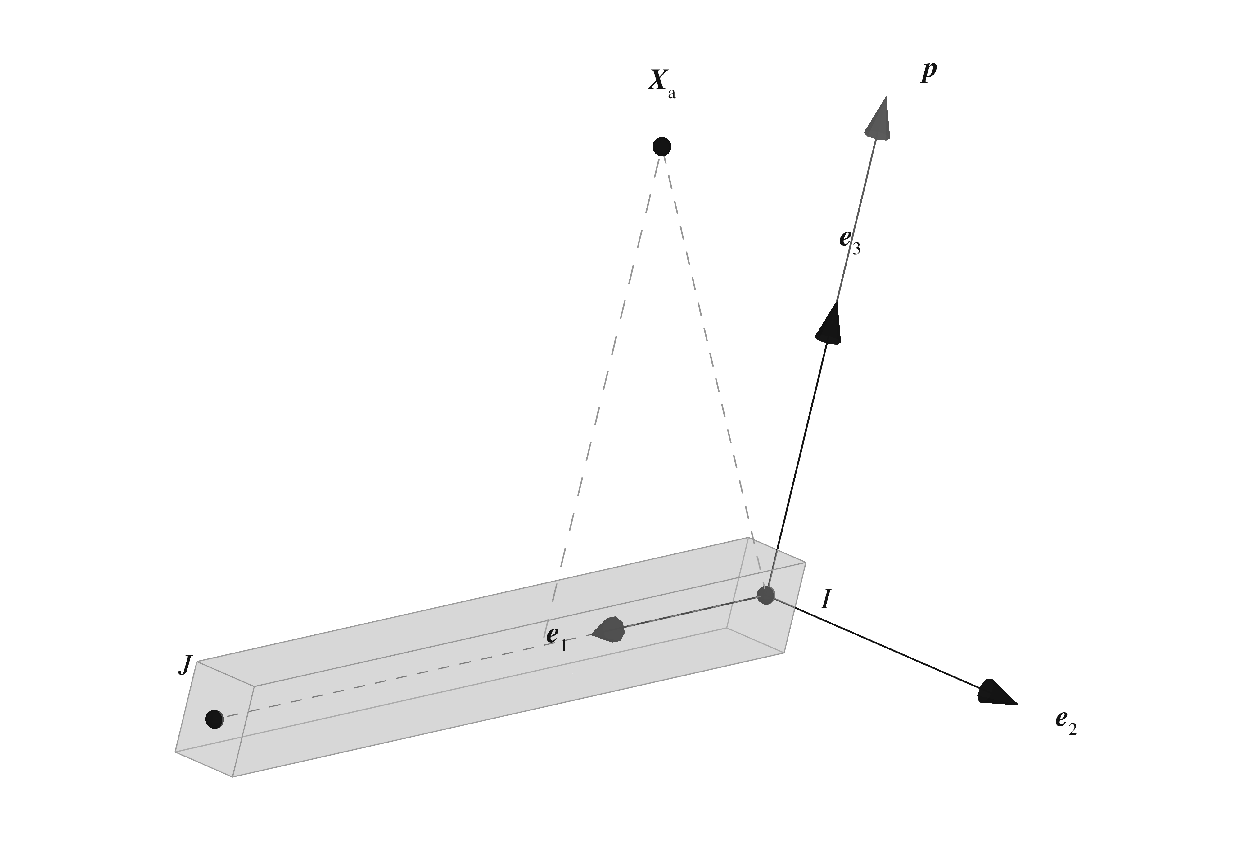
\includegraphics[width=.96\linewidth,height=.40\textheight,keepaspectratio]{figures/tecplot/concept_elemento.pdf}
\caption[Discretización y sistema local del elemento]{Orientación espacial de un elemento entre los nodos $I$ y $J$. El punto auxiliar $\vct X_a$ define una dirección transversal mediante su proyección $\vct p$ sobre el plano normal a $\vct e_1$. $\vct e_3$ es paralelo a $\vct p$ y $\vct e_2=\vct e_3\times\vct e_1$. El punto auxiliar no añade grados de libertad.}\label{fig:elemento}
\end{figure}

Sean las columnas de $\ten Q_e$ los ejes locales expresados en el sistema de referencia
newtoniano $\mathcal F_N$. Entonces $\vct v^N=\ten Q_e\vct v^e$ y
\begin{equation}
 \vct q_e=\ten T_e\vct q_e^N,\qquad
 \ten T_e=\diag(\ten Q_e^{\tr},\ten Q_e^{\tr},
                    \ten Q_e^{\tr},\ten Q_e^{\tr}).
\end{equation}
En una configuración fijada, $\ten K_e^N=\ten T_e^{\tr}\ten K_e\ten T_e$,
$\ten M_e^N=\ten T_e^{\tr}\ten M_e\ten T_e$ y
$\vct f_e^N=\ten T_e^{\tr}\vct f_e$. Son cambios de componentes, no
aproximaciones adicionales. Si la base gira, las ecuaciones dinámicas requieren
además las derivadas temporales de la transformación, como se explicita más adelante.

La matriz de conectividad $\ten L_e$ extrae del vector global $\vct q$ las
coordenadas del elemento: $\vct q_e^N=\ten L_e\vct q$. El ensamblaje suma
contribuciones que realizan trabajo sobre las mismas coordenadas:
\begin{equation}
 \ten K=\sum_e\ten L_e^{\tr}\ten K_e^N\ten L_e+\ten K_{\rm uniones},
 \qquad
 \ten M=\sum_e\ten L_e^{\tr}\ten M_e^N\ten L_e+\ten M_{\rm cuerpos}.
\end{equation}
Las masas de góndola y cubo y las leyes del tren o la base se incorporan
mediante sus relaciones de conexión. La coincidencia espacial de dos puntos no
impone por sí sola igualdad de desplazamientos: debe existir una conectividad
compartida o una restricción declarada.

\section{Vínculos entre el cubo y las raíces de las palas}

Se utiliza el punto de referencia del cubo como maestro cinemático; las raíces
son puntos dependientes. ``Maestro'' y ``esclavo'' describen la elección de
coordenadas independientes y no una dirección única de transmisión de fuerzas.
Las reacciones en las raíces también producen resultantes sobre el cubo.

\begin{figure}[htbp]
\centering
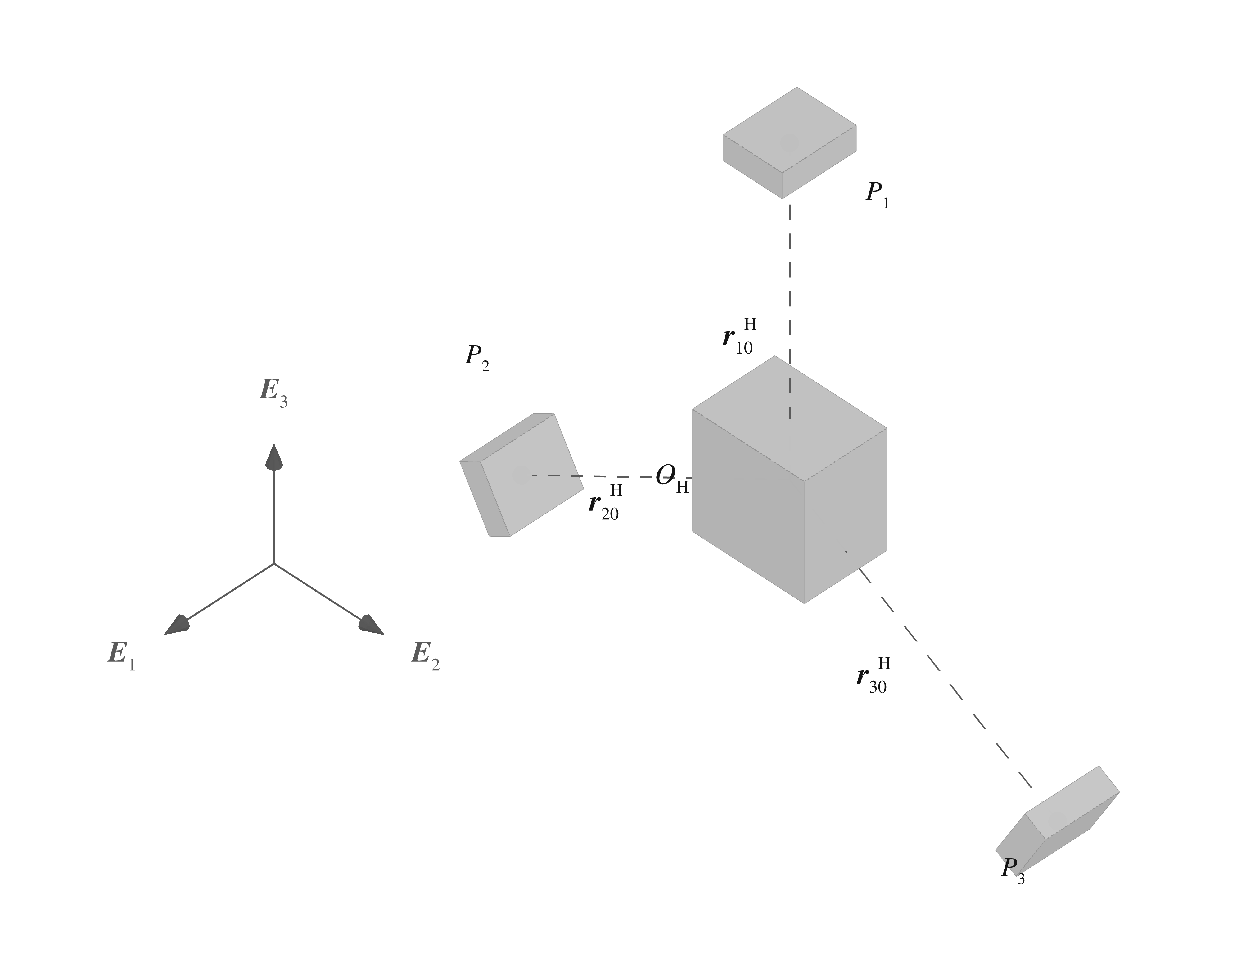
\includegraphics[width=.96\linewidth,height=.40\textheight,keepaspectratio]{figures/tecplot/concept_cubo-brazos.pdf}
\caption[Vínculo rígido entre el cubo y las raíces]{Brazos nominales $\vct r_{b0}^H$ desde el origen del cubo hasta las tres raíces $P_b$. Las líneas discontinuas distinguen estas relaciones geométricas de los volúmenes ilustrativos. Las separaciones son esquemáticas y no indican elementos flexibles adicionales.}\label{fig:cubo-brazos}
\end{figure}

Sea $\vct r_{s0}$ el brazo constante expresado en $\mathcal F_H$ y
$\ten Q_H={}^{N}\ten Q_H$ la orientación actual del cubo. La relación exacta
de posiciones es
\begin{equation}
 \vct x_s=\vct x_H+\ten Q_H\vct r_{s0}.
 \label{eq:fe-rigido-exacto}
\end{equation}
Para un vínculo soldado, la orientación de la raíz difiere de la del cubo
solo por una rotación de montaje constante. Si se permite una articulación
de paso, debe introducirse otra coordenada relativa; no se describe con el
vínculo soldado utilizado aquí.

Al variar \eqref{eq:fe-rigido-exacto}, expresando las rotaciones incrementales
en el mismo sistema de referencia $N$ y definiendo $\vct r_s=\ten Q_H\vct r_{s0}$, se obtiene
\begin{equation}
 \delta\vct u_s=\delta\vct u_H+
 \delta\vct\theta_H\times\vct r_s,
 \qquad \delta\vct\theta_s=\delta\vct\theta_H.
 \label{eq:desplazamiento-raiz}
\end{equation}
Por tanto,
\begin{equation}
 \delta\vct q_s=\ten B_s\delta\vct q_H,
 \qquad
 \ten B_s=\begin{bmatrix}\Id&-\sk{r_s}\\0&\Id\end{bmatrix}.
 \label{eq:compatibilidad-incremental}
\end{equation}
El brazo produce el desplazamiento de la raíz asociado a la rotación del
cubo; suprimirlo conserva solo una parte de la compatibilidad. La igualdad de
rotaciones incrementales presupone componentes comunes, no igualdad de
ángulos de Euler definidos en bases diferentes.

La suma vectorial de la figura~\ref{fig:vinculo-raiz} muestra por qué las traslaciones de una raíz y del punto maestro no son, en general, iguales. Incluso si el cubo no se traslada, su pequeña rotación desplaza una raíz situada a una distancia finita del eje. El término $\delta\vct\theta_H\times\vct r_s$ representa ese desplazamiento compatible, no una deformación del brazo.
\begin{figure}[htbp]
\centering
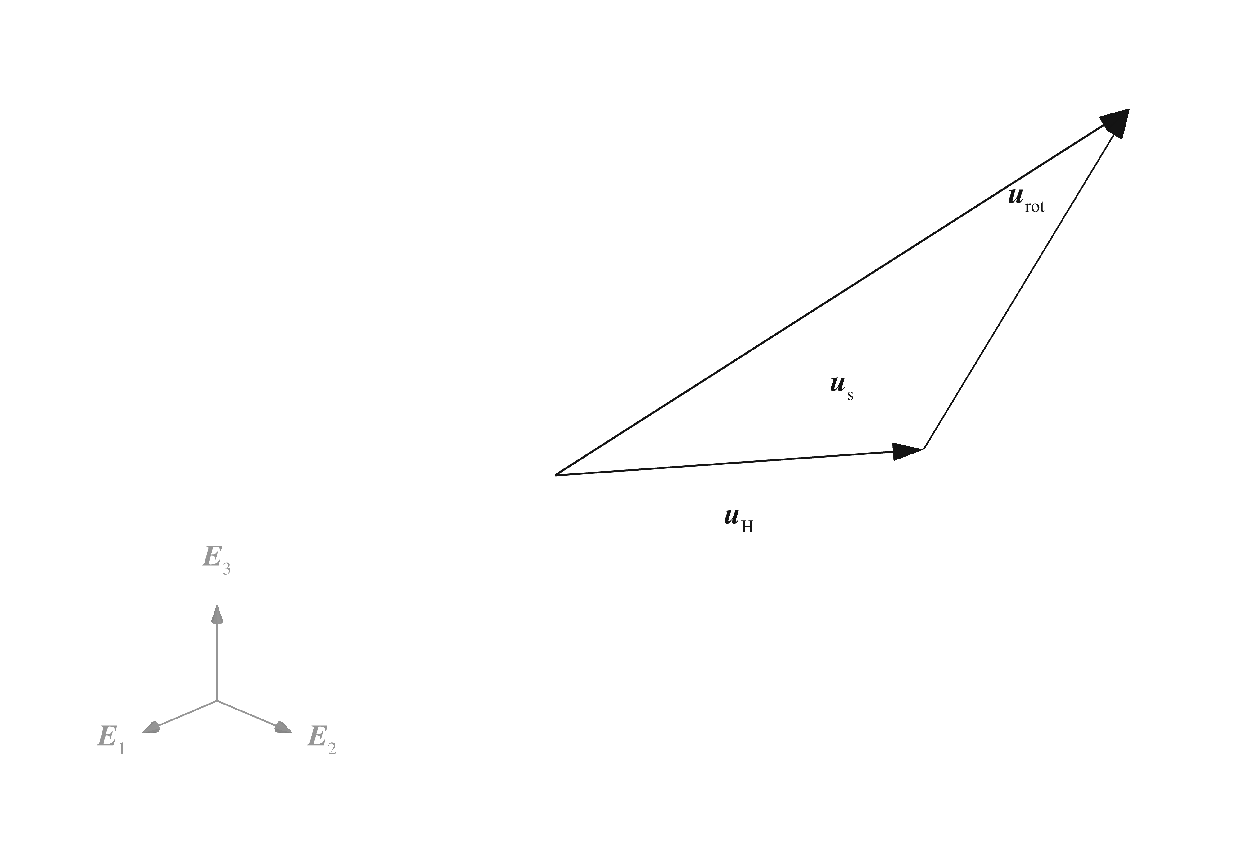
\includegraphics[width=.96\linewidth,height=.40\textheight,keepaspectratio]{figures/tecplot/concept_vinculo-raiz.pdf}
\caption[Desplazamiento compatible de una raíz]{Compatibilidad incremental de una raíz: $\vct u_s=\vct u_H+\vct u_{rot}$, donde $\vct u_{rot}=\vct\theta_H\times\vct r$. La suma se representa mediante flechas consecutivas y la flecha directa cierra el desplazamiento total. El punto intermedio corresponde solamente a la traslación común del cubo.}\label{fig:vinculo-raiz}
\end{figure}

\subsection{Restricciones dependientes del tiempo}

En el movimiento nominal de giro prescrito, los brazos expresados en $N$
varían aunque sean constantes en $H$. Para eje fijo,
\begin{equation}
 \dot{\vct r}_s=\sk{\Omega}\vct r_s,\qquad
 \ddot{\vct r}_s=\sk{\Omega}^{2}\vct r_s.
\end{equation}
Estas derivadas ocupan el bloque superior derecho de $\dot{\ten B}_s$ y
$\ddot{\ten B}_s$, con el mismo signo negativo. Si se reúnen los vínculos en
$\delta\vct q=\ten T(t)\vct z$, las velocidades y aceleraciones son
\begin{align}
 \delta\dot{\vct q}&=\ten T\dot{\vct z}+\dot{\ten T}\vct z,\\
 \delta\ddot{\vct q}&=\ten T\ddot{\vct z}
 +2\dot{\ten T}\dot{\vct z}+\ddot{\ten T}\vct z.
\end{align}
Sustituirlas en
$\ten M\delta\ddot{\vct q}+\ten D\delta\dot{\vct q}
+\ten K\delta\vct q=\delta\vct f$
y proyectar mediante $\ten T^{\tr}$ proporciona
\begin{align}
 \ten M_r&=\ten T^{\tr}\ten M\ten T,\\
 \ten D_r&=\ten T^{\tr}(\ten D\ten T+2\ten M\dot{\ten T}),\\
 \ten K_r&=\ten T^{\tr}(\ten K\ten T+\ten D\dot{\ten T}
 +\ten M\ddot{\ten T}),\\
 \vct f_r&=\ten T^{\tr}\delta\vct f.
 \label{eq:fe-reduccion-temporal}
\end{align}
Las reacciones ideales desaparecen de la ecuación proyectada porque no
realizan trabajo virtual sobre movimientos admisibles. Esta eliminación es
exacta dentro de las restricciones linealizadas y no equivale a truncar modos.
Una congruencia estática basta únicamente cuando $\dot{\ten T}=0$ y
$\ddot{\ten T}=0$. Elegir un azimut de evaluación no anula esas derivadas.

Los empotramientos y movimientos impuestos de la base $\mathcal F_B$ se
tratan asimismo como condiciones cinemáticas. Para una condición no homogénea
se escribe $\delta\vct q=\ten T\vct z+\vct q_p(t)$, y sus derivadas producen
la carga equivalente correspondiente. Así quedan separados los grados de
libertad estructurales, las coordenadas eliminadas por compatibilidad y los
movimientos prescritos. Esta separación es la base para introducir, en el
capítulo siguiente, el estado de operación y las ecuaciones de sus perturbaciones.

\section{Conexión elástica entre la góndola y el rotor}
La unión entre la góndola y el cubo transmite acciones que dependen de su movimiento relativo. Para pequeñas perturbaciones, sean $\vct u_G,\vct\theta_G$ y $\vct u_H,\vct\theta_H$ las traslaciones y rotaciones de los dos puntos de referencia, expresadas en una base común. El vector $\vct d$ une esos puntos en el estado alrededor del cual se linealiza. La deformación relativa se escribe
\begin{equation}
 \vct\Delta_d=
 \begin{bmatrix}
 \vct u_H-\vct u_G-\vct\theta_G\times\vct d\\
 \vct\theta_H-\vct\theta_G
 \end{bmatrix}
 =\mathsf B_d\vct q.
 \label{eq:conexion-elastica}
\end{equation}
El término $\vct\theta_G\times\vct d$ es el desplazamiento que tendría el punto del cubo si siguiera rígidamente la perturbación de la góndola. Restarlo permite medir únicamente el movimiento relativo que deforma la conexión. En particular, un movimiento de cuerpo rígido común a ambos componentes produce $\vct\Delta_d=\vct0$.

La figura~\ref{fig:conexion-elastica} representa las acciones de la conexión mediante un resorte y un amortiguador equivalentes. Estos símbolos sintetizan las relaciones entre las seis componentes relativas, no solo una traslación axial.

\begin{figure}[htbp]
\centering
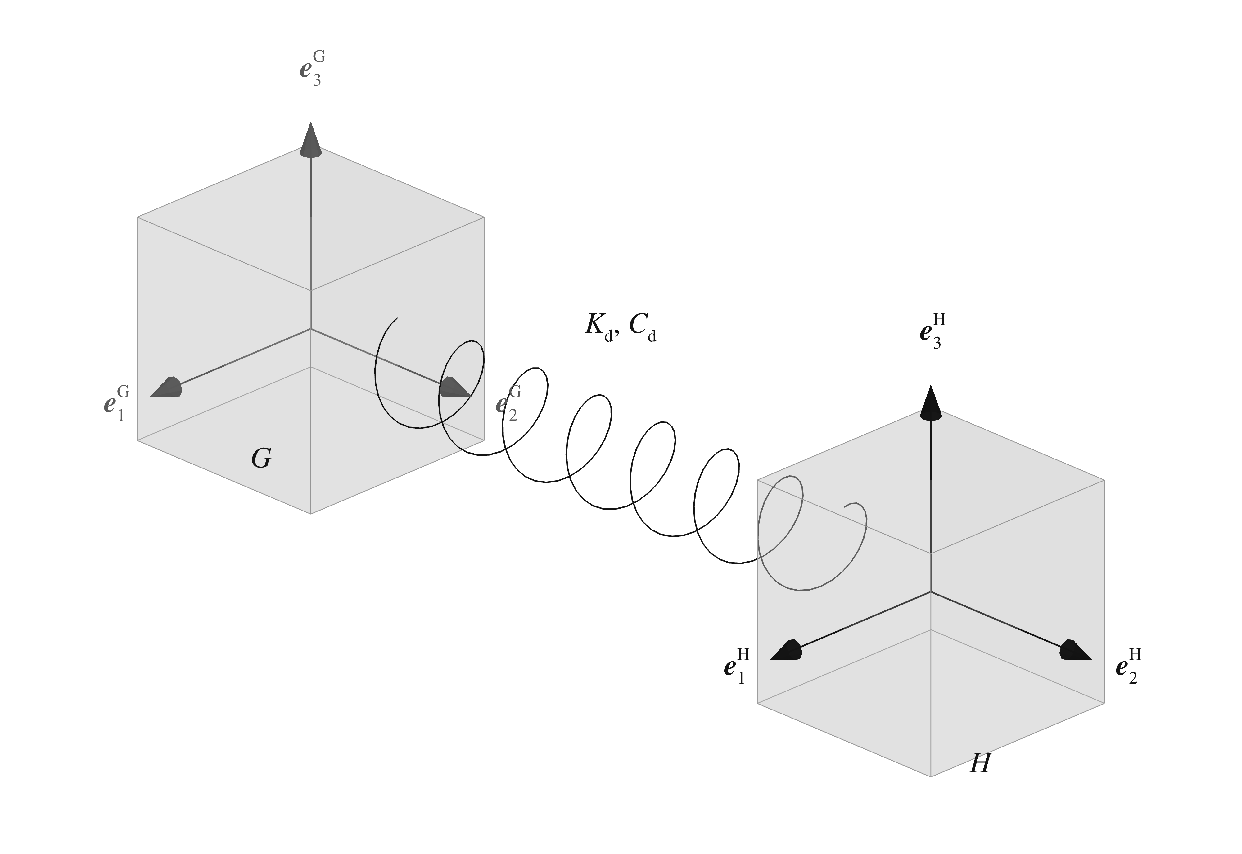
\includegraphics[width=.96\linewidth,height=.40\textheight,keepaspectratio]{figures/tecplot/concept_conexion-elastica.pdf}
\caption[Conexión elástica entre góndola y rotor]{Conexión elástica entre los sistemas de la góndola y el cubo. El resorte representa de forma simbólica los operadores generalizados de rigidez $K_d$ y disipación $C_d$. No implica un único grado de libertad ni fija la geometría de un cojinete comercial.}\label{fig:conexion-elastica}
\end{figure}

Con matrices de rigidez y amortiguamiento de conexión $\mathsf k_d$ y $\mathsf c_d$, las acciones conjugadas a $\vct\Delta_d$ son $\mathsf k_d\vct\Delta_d$ y $\mathsf c_d\dot{\vct\Delta}_d$. Para una matriz $\mathsf B_d$ constante, sus contribuciones al sistema son
\begin{equation}
 \mathsf K_d=\mathsf B_d^\tr\mathsf k_d\mathsf B_d,\qquad
 \mathsf C_d^{\,\mathrm{unión}}=\mathsf B_d^\tr\mathsf c_d\mathsf B_d.
\end{equation}
Si la base elegida hace que $\mathsf B_d$ dependa del tiempo, se conserva
$\dot{\vct\Delta}_d=\mathsf B_d\dot{\vct q}+\dot{\mathsf B}_d\vct q$.
La rigidez torsional de la conexión actúa sobre la desviación angular respecto del giro nominal. Una rigidez positiva produce una oscilación torsional elástica; no constituye un modo de cuerpo rígido.

